\section{Plany rozwoje lub obecnie implementowane}
\label{chapter:application:plans}

Aplikacja do zarządzania logami jest w fazie aktywnego rozwoju. 
Do tej pory udało się osiągnąć relatywnie prostą architekturą, dzięki której
możliwe jest zbieranie logów ze wskazanych maszyn oraz opisania ich
dodatkowymi danymi, pozwalającymi łatwo zidentyfikować skąd i kiedy
zostały pobrane oraz wskazać na ich znaczenie w kontekście monitorowanego systemu.
Przedstawione poniżej, elementy, są na obecną chwilę rozwijane i dotyczą aplikacji, programów
oraz zagadnień, która znajdują w zakresie przetwarzania logów. Niemniej, poza tym, autor
pracy dyplomowy, bierze, oraz brał, aktywny udział w tworzenia, projektowania i dyskusji
dotyczących innych części końcowego produktu. Z uwagi na zawodowy charakter opisywanych rozwiązań, nie
jest możliwe zaprezentowania oraz omówienie szczegółów na odpowiednim poziomie szczegółowości. 
Niemniej dotyczą ona zagadnień takich jak:
\begin{itemize}
    \item tworzenia klastrów dla poszczególnych aplikacji całego systemu,
    \item automatyzacji powyższych operacji,
    \item \textbf{multi-tenancy} w postaci wtyczki dla aplikacji \textbf{Kibana},
    \item przenoszenia, poza \textbf{monasca-log-api}, kolejnych komponentów do języka Python,
    \item korelowania metryk oraz informacji zebranych z logów
\end{itemize}

\subsection{Alarmy a logi}
\label{chapter:application:plans:alarm_on_logs}

Jednym z głównych założeń projektu \textbf{monasca} jest powiadamiania użytkownika o 
sytuacjach krytycznych zaistniałych w systemie. Funkcjonalność realizowana jest na podstawie
metryk, zbieranych z całego systemu. Przekroczenie, założonych przez administratora, wartości
krytycznych, skutkuje wygenerowaniem alarmu. Jednak idea ta, nie może zostać
tak łatwo przełożona na logi. 

    \subsubsection{Idea implementacji}
    \textbf{monasca-agent} jest programem, którego głównym zadaniem jest zbierania metryk z systemu, na którym
    został on zainstalowany. Podejście takie sprawdza się w pełni i właściwie jest jedynym możliwym rozwiązaniem,
    jeśli chodzi o monitoring stanu systemu operacyjnego, maszyny lub aplikacji na nim uruchomionych. Niekoniecznie,
    jest to jednak podejście właściwie dla podobnej analizy w przypadku logów. W rozwiązaniu typu \textbf{LaaS}, 
    jednym z celów jest przesłanie danych do centralnej lokalizacji - archiwizacja. W tym samym punkcie, lub
    przesłane dalej, są one podmiotem analizy. Implementacja będzie, przynajmniej koncepcyjne, zbliżona do \textbf{monasca-agent}.
    
    Możliwe są dwie implementacja:
    \begin{itemize}
        \item[dynamiczna] - potencjalny program miałby być zlokalizowany w za \textbf{monasca-log-transformer} (\ref{chapter:monasca:monasca_log_transformer}).
        Odbierałby on logi ze wspomniane programu, które wysyłane byłyby na ten sam lub inny \glslink{kafka_topic}{\textbf{topic}} i poddawał je prostej analizie. 
        \item[statyczna] - oparta o okresowe pobierania relatywnie małych ilości danych z bazy ElasticSearch (\ref{chapter:application:elkstack:elasticsearch}). 
        Zapytanie oczywiście byłoby zoptymalizowanie na pobranie jedynie tych rekordów, gdzie poziom logu osiągnął zadaną przez operatora wartość.
    \end{itemize}
    
    \subsubsection{Analiza dynamiczna w strumieniu}
    \label{chapter:application:plans:alarm_on_logs:streaming}
    
    \begin{figure}[H]
        \centering
        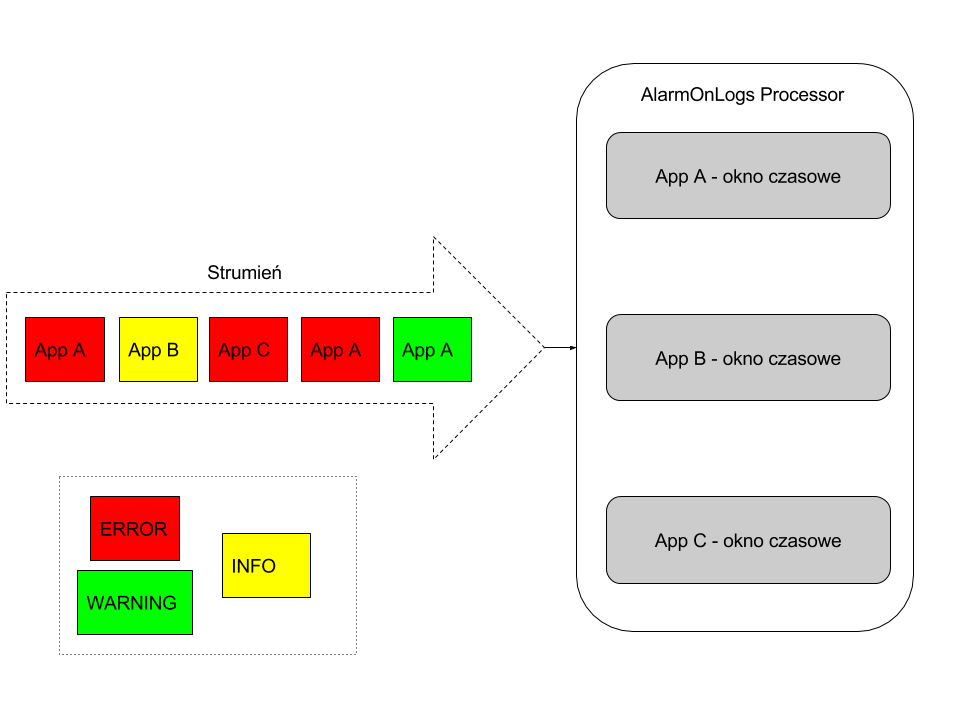
\includegraphics[width=1.0\textwidth]{images/aol_stream}
        \caption[Analiza w strumieniu - schemat]{
            Analiza w strumieniu - schemat, 
            źródło: opracowanie własne
        }
        \label{chapter:application:plans:alarm_on_logs:streaming:diagram}
    \end{figure}
    
    Jest to alternatywa, która idealnie wpisuje się w rzeczywisty charakter danych, jakimi są logami. Ponadto, jest to rozwiązanie, w którym
    wyeliminowana zostaje konieczność iterowanie po zbiorach danych, których wielkość może znacząco spowalniać proces analizy. W programowaniu,
    pętle są najczęściej wskazywane jako najwolniejsze elementy aplikacji, chociaż oczywiście momentami nie da się ich uniknąć. Ponadto, nie ma 
    konieczności także okresowego pobierania danych, co znacząco wydłuża czas odpowiedzi program. Pod uwagę należy jednak wziąć pewne punkty wymagania,
    które musiałyby być spełnione, a które są wyznacznikami przetwarzania w czasie rzeczywistym.
    \begin{itemize}
        \item[ciągły przepływ] - dane, zgodnie z filozofią przetwarzania strumieniowego, muszą przepływać przez aplikację. Wynika z tego, że szybkość
        przetwarzania jest tutaj nadrzędnym celem do osiągnięcia,
        \item[przeciwdziałania strumieniowi] - mimo, że brzmi to jak jeden z antywzorców programowania,
        \footnote{\textbf{Fighting against framework} - próba celowego wykorzystania biblioteki lub wzorca do zadań, do których nie został on zaprojektowany},
        jest to ważna cecha przetwarzania danych w czasie rzeczywistym. Podobnie, jak w rzeczywistym potoku, dane, jak ryby, mogą pływać ławicami, ale mogą
        również napływać pojedynczo, w określonych, i co ważne - nieregularnych, odstępach czasu. Ważne jest więc, aby nie blokować programu, w oczekiwaniu
        na dane. Rozwiązaniem jest zastosowanie mechanizmów takich jak okna przesuwne, których działania powinno się zakończyć po określonym upływie czasu lub
        aktywne nasłuchiwania na pojawiające się dane na wejściu. Szczęśliwie, istnieje odpowiednie biblioteki, które realizuję funkcję aktywnego oczekiwania,
        i wznawiają właściwy wątek programu, jeśli takowa wiadomość nadejdzie. Z drugiej strony, dane mogą napływać dużo szybciej niż aplikacja jest w stanie
        je przetworzyć. W tym wypadku, konieczne może okazać się minimalne buforowanie danych lub przetwarzanie napływających informacji w sposób równoległy.
        \item[powtarzalne rezultaty] - aby silnik alarmujący na podstawie logów generował powtarzalne i, przede wszystkim, 
        spójne rezultaty konieczne jest, aby dane analizować, nie tyle pod kątem poziomu logu, ale także pod względem czasu w jakim został on wygenerowany. 
        Jest to szczególnie istotne, ponieważ system generujący alarm na podstawie tylko jednego punktu wykraczającego poza skalę byłby 
        narażony na zgłaszanie zbyt dużej liczby fałszywych alarmów. Innymi słowy, jeśli system wykryje n-krotne powtórzenie 
        niepoprawnej wartości, powinien wtedy, i tylko wtedy wygenerować alarm. 
        Co prawda, w przypadku logów, omówiona sytuacja, nie zawsze musi być prawdą. Jednostkowe przekroczenie zużycia procesora, nie jest sytuacją anormalną.
        Niemniej, tylko jeden błąd zalogowany przez aplikację o krytycznym znaczeniu może oznaczać błąd. Ale, jeśli program zapisuje w logach jedynie ostrzeżenia,
        dopiero pewna ich liczba, zaobserwowana w, przykładowo, ostatnich 10 minutach działania aplikacji, może zostać uznana, ze problem. Jeśli dane, nie byłyby
        przeglądane pod kątem czasu, w którym powstał wpis, rezultaty analizy byłyby nierzetelne. 10 krotne zaobserwowania wartości \textbf{WARNING} mogłoby tak naprawdę
        pochodzić z próbek wygenerowanych w ciągu ostatnich 30 minutach, a sam fakt, zgłoszenia błędu spowodowany tym, że dotarły one do silnika analizującego
        w oknie czasowym o długości co najwyżej 10 minut \cite{8_requirements_of_real_time_processing}.
        \item[grupowanie] - nie jest to problem, jeśli analizuje się zbiór danych. W danej próbce kontrolnej, dane można łatwo posortować i na jej podstawie 
        wygenerować pewien wynik. Sytuacja komplikuje się dla danych przetwarzanych w potoku. Potencjalny silnik alarmujący otrzymywałby dane pochodzącego z,
        potencjalnie, nieskończonej, liczby różnych programów. Operator, mógłby tak skonfigurować alarmy, aby wykrywać 5 krotne pojawienie się wartości \textbf{ERROR}
        dla aplikacji A, w ciągu 5 minut. Innymi słowy, aplikacja analityczny, musiałaby zapamiętać pojawienia się pierwszego wystąpienia problematycznej wartości.
        Kolejny wymogiem byłoby monitorowanie czasu, jaki upłynął od momentu zauważania wartości po raz pierwszy. Ostatecznie, wygenerowania odpowiedniego,
        alarmu powinna ograniczać się do tych wartości, które wykryto jedynie dla konkretnej aplikacji.
    \end{itemize}
    
    \subsubsection{Analiza tradycyjna na zbiorze}
    \label{chapter:application:plans:alarm_on_logs:bulk}
    
    \begin{figure}[H]
        \centering
        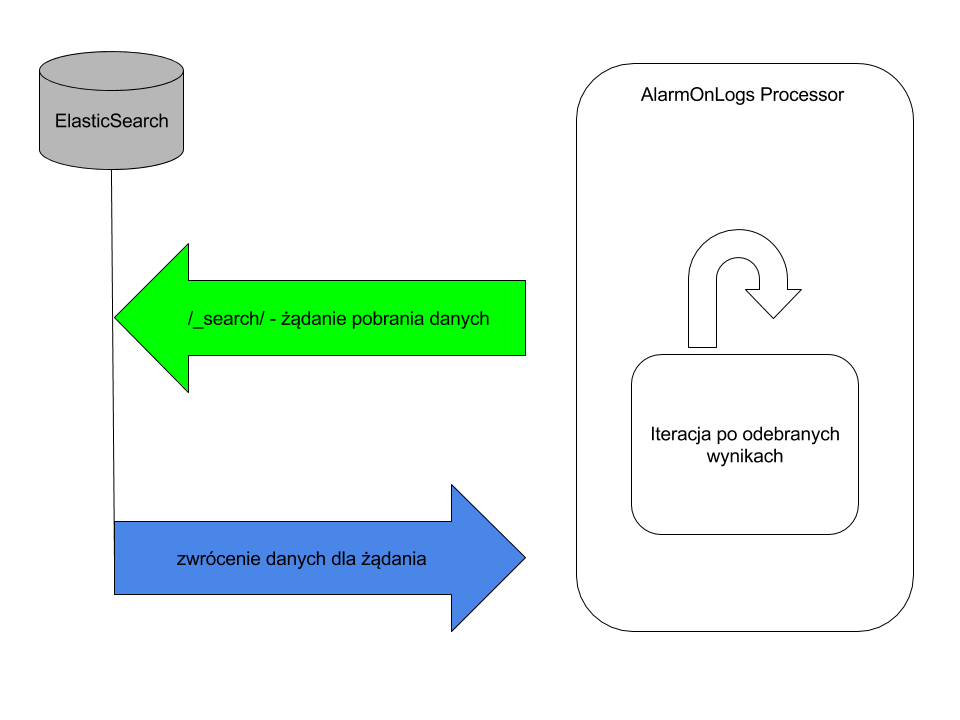
\includegraphics[width=1.0\textwidth]{images/aol_batch}
        \caption[Analiza na zbiorze - schemat]{
            Analiza na zbiorze - schemat, 
            źródło: opracowanie własne
        }
        \label{chapter:application:plans:alarm_on_logs:bulk:diagram}
    \end{figure}
    
    Rozwiązanie alternatywne do omówionego w \ref{chapter:application:plans:alarm_on_logs:streaming}. Rozwiązuje ono wszystkie, przedstawione
    wyżej wymaganie, jakie musiałby spełnić silnik alarmujący, łącznie z grupowaniem. Aplikacja mogłaby pobierać dane, w określonym oknie czasowym,
    ze wskazaniem na poziomu logów oraz aplikacje. Jeśli w odebranych wynikach znalazłyby się odpowiednia
    ilość rekordów, gdzie wartości byłyby przekroczone, byłby to sygnał do wygenerowania alarmu. Niemniej, rozwiązanie tego typu, cechuje się
    narzutem wynikającym z:
    \begin{itemize}
        \item konieczność wygenerowania żądania, otrzymania odpowiedzi i ostatecznie rozpakowania danych do postaci, w której mogłyby zostać
        przetworzone,
        \item program nie może pobierać danych zbyt szybko. Pomijając fakt, że mogłoby to negatywnie wpłynąć na jej wydajność bazy danych, która
        musiałaby przeznaczyć więcej zasobów, aby zrealizować żądanie, wynikałoby to również z konieczności zakończenie przetwarzania już
        otrzymanych danych,
        \item program operowałby na zbiorze, o zmiennej wielkości. Nie byłoby, oczywiście, problematyczne zweryfikowanie małego lub pustego zbioru,
        niemniej otrzymanie dużej ilości rekordów, przełożyłoby się na łączne (czas przesłania, przetworzenia do zrozumiałego formatu, iteracji)
        wydłużenia czasu operacyjnego zaszytego algorytmu. 
    \end{itemize}
    W środowisku, gdzie konieczne jest, szybkie reagowania na ciągle zmieniające się warunki, jakiekolwiek opóźnienia są same w sobie, źródłem
    problemu. Niemniej rozwiązanie to, ma tę szczególną zaletę, że opiera się na istniejącej bazie danych o rozbudowanym API, zdolnym
    zwrócić dane w kompaktowej formie.
    
    Poboczną zaletą obu rozwiązań, jeśli wybranego by oddzielny topic przeznaczony jedynie dla programów analizujących dane, byłoby wykreowania
    swoistej tablicy trasowania (działającej na zasadzie zbliżonej do tej znanej z urządzeń sieciowych), co w dalszej kolejności mogłoby
    służyć do rozdysponowania przekształconych logów do różnych punktów docelowych, gdzie stałyby się one podmiotem całkowicie odrębnych operacji.
    Program miałby za zadania analizować zawartość przesłanych logów. Jeśli poziom, którekolwiek z nich przekroczył by zadaną (skonfigurowaną przez
    administratora lub operatora) wartość, aplikacja tworzyłaby odpowiednią metrykę.
    Obie z implementacji zostały zaproponowane przez autora pracy dyplomowej jako przeciwne do siebie, łącznie z ich zaletami oraz wadami.

    \subsubsection{Metryki nieciągłe}
    W obu przypadkach, niezależnie od przyjętej implementacji, problem jest przedstawienie zebranych danych w postaci metryk - czyli wartości
    numerycznych. W przeciwieństwie do danych dotyczących, chociażby, zużycia przestrzeni dyskowej lub, podlegającemu większej
    fluktuacji, obciążeniu procesora, logi stanowią element zbioru metryk nieciągłych \footnote{Sparse metric - metryki okresowe,
    zwracające wartości w nieregularnych odstępach czasu}. Częścią rozwiązania problemu, byłaby modyfikacja aplikacji \textbf{monasca-thresh},
    odpowiedzialnej za faktyczne generowania alarmów. Na obecną chwilę, jeśli dla danej metryki, brak jest danych, monitor zdefiniowany
    dla danego alarmu powoduje jego wejście w stan \textbf{UNDETERMINED}. W przypadku logów, nie jest to jednak sytuacja oczekiwana. 
    Przykładowo, brak wystąpień błędów dla danej aplikacji, powinien faktycznie oznaczać, że aplikacja lub system pracuje poprawnie i
    potencjalny operator nie ma powodów do niepokoju. Innymi słowy, odpowiadałoby to stanowi \textbf{OK}. Dopiero, co najmniej jedna wartość
    wykraczająca poza ramy danego alarmu, powinna spowodować jego przejście w stan wysoki oraz wygenerowanie powiadomienia lub powiadomień.
\newglossaryentry{healthcheck}{
    name={Healthcheck},
    description={
        Specjalny adres, dostępny w \textbf{REST}'owym API, który informuje odpytującego o stanie aplikacji. Zależnie
        od implementacji, można wyróżnić co najmniej dwa typy tego rodzaju komponentów:
        \begin{itemize}
            \item[proste] - informujące jedynie o tym, czy API jest dostępne i można wykonywać żądania,
            \item[złożone] - oferujące tą samą funkcjonalność co \textit{proste} oraz, dodatkowo,
            weryfikujące stan zależnych serwisów, jak chociażby baza danych.
        \end{itemize}
    }
}
\newglossaryentry{loadbalancer}{
    name={Load Balancer},
    description={
        Rodzaj aplikacji, najczęściej znajdujący się przed klastrem serwerów. Jego nadrzędnym zadaniem jest
        dystrybuowanie ruchu do poszczególnych węzłów według zadanego algorytmu. Operacja ta ma na celu,
        równomiernie rozłożenie obciążenia, które generowane jest przez klientów, łączących się do klastra
    }
}

\subsection{Healthcheck}
\label{chapter:application:plans:healthcheck}

Mechanizmy oferowane przez \glslink{healthcheck}{\textbf{healtcheck}'i} dostępne są, na obecną chwilę, jedynie
w następujących aplikacjach: \textbf{monasca-api} oraz \textbf{monasca-log-api}. Dodatkowo, są to wersje napisane w języku
Java. Biorąc pod uwagę trend w społeczności \textbf{monasca} dążący do przejścia na wersje napisane w języku Python,
autor, poniższej pracy dyplomowej, stworzył propozycję implementacji na potrzeby \textbf{monasca-log-api}. Dzięki
temu, możliwe jest wysyłanie żądań do serwera, na które odpowiedzieć on może w następujący sposób:
\begin{itemize}
    \item[HTTP 204] - oznacza, że \textbf{monasca-log-api} działa oraz \textbf{Kafka}, które wykorzystywane jest
    do przysyłania danych do \textbf{monasca-log-transformer} jest również obecne w sieci, a wymagane \glslink{kafka_topic}{topic'i} są
    utworzone
    \item[HTTP 503] - komponent zależny - kafka - jest niedostępna lub niepoprawnie skonfigurowana,
    \item[HTTP 404] - \textbf{monasca-log-api} jest niedostępny
\end{itemize}

Całość została oparta o bibliotekę \textbf{oslo.middleware}. Warto dodać, że ta oraz inne biblioteki, których nazwa
rozpoczyna się od \textbf{oslo.} są, praktycznie, nieodłączną częścią chmury obliczeniowej \textbf{OpenStack}. Z tego też powodu,
są wykorzystywane w bardzo dużej liczbie projektów i to nie tylko tych, które stanowią główną część \textbf{OpenStack} (jak chociażby
\textbf{Horizon czy \textbf{Nova}}).

Dodatkowo autor pracy dyplomowej, zajął się zweryfikowaniem możliwych alternatyw dla omawianego
rozwiązania. Problematyczna okazuje się, bowiem, jedna różnica między wersjami napisanymi w językach \textbf{Python} oraz \textbf{Java}.
Implementacja oparta o język \textbf{Java} wykorzystuję bibliotekę \textbf{DropWizard}, która domyślnie wspiera funkcjonalność określaną
nazwą \textit{healthcheck}. Dodatkowo, serwer uruchamia kolejną (wbudowaną) usługę dostępną pod innym portem.
Jest to duża zaleta w momencie kiedy \textbf{API} umieszcza się wraz z innymi jego instancjami, a gdzie wszystkie umieszczone są
za specjalnym koordynatorem ruchu - \glslink{loadbalancer}{\textbf{loadbalencer}'em}. Posiadanie \textbf{healtcheck} poza głównym API, pozwala
na wydzielenie tych żądań spoza zakresy pracy \textbf{loadbalencer}. Niestety, biblioteki dostępne w \textbf{Python} nie dają takich możliwość.
Również próby uruchomienia wbudowanego serwera WSGI, działającego na innym porcie, okazały się nieskuteczne. Dużym problem okazał się
sposób pracy serwera \glslink{wsgi}{WSGI} wybranego przez społeczność - Gunicorn. W momencie załadowania kompletnej aplikacji, Gunicorn
wchodzi w pętlę, której nadrzędny wątek jest blokujący i wznawiany w momencie otrzymania żądania. Przez to uruchomiony wewnętrznie serwer, nie
pozwala na uruchomienie właściwej aplikacji. Rozwiązaniem wydawałoby się więc wystartowanie go wywnętrz oddzielnego procesu, działającego równoległe
do głównego wątku API. Niestety, przy tym podejściu, niemożliwe jest poprawne wyłączenie zarówno wątku \textbf{healthcheck} oraz \textbf{API}.
Biorąc pod uwagę te problemy oraz możliwości oferowane przez \textbf{oslo.middleware}, omawiana funkcjonalność została zrealizowana jako filtr,
uruchamiany przed faktyczną logiką biznesową. 

Propozycja implementacji dostępna jest pod adresem \url{https://review.openstack.org/#/c/249685/} i oczekuje na akceptację 
społeczności lub dalsze usprawnienia.
\section{Wiele logów dla monasca-log-api (bulk-mode)}
\label{chapter:application_own:plans:bulk_monasca_log_api}

W pierwszych słowach warto nadmienić, że opisana w poniższym rozdziale funkcjonalność oryginalnie została 
zaproponowana zanim zespół, którego autor pracy dyplomowej jest członkiem, rozpoczął właściwie prace
nad implementacją kolejnych elementów, wchodzących w skład całego systemu. Na obecną chwilę, z ideą 
dodania trybu \textbf{bulk} do \textbf{monasca-log-api}, wyszła firma \textbf{TSV}, która zauważyła brak tej
ważnej funkcjonalności. Interesującym jest, że ten sam fakt, autor oraz inni członkowie zespołu, zauważyli
w tym samym momencie. 

Ideą całego rozwiązania będzie możliwość przesyłania z \textbf{monasca-log-agent} wielu zebranych logów
w jednym żądaniu. Poprzez to cały proces przetwarzania zostanie przyspieszony i ostatecznie logi
będzie można analizować szybciej. Szybsza analiza wiąże się również z szybszym zapisaniem logów w centralnej lokalizacji,
a tym samym zabezpieczeniem całego systemu przed ich utratą. Autor pracy dyplomowej jest jedną z dwóch osób, które będą
współpracowały z firmą TSV na wymienionych poniżej płaszczyznach:
\begin{itemize}
    \item akceptacja zaproponowanego przez TSV planu implementacji,
    \item zaproponowanie koniecznych zmian, które należy wprowadzić do istniejącej implementacji \textbf{monasca-log-api}
    w kontekście adresów pod którymi dostępna będzie logika, a na które będzie można wysyłać logi,
    \item ocenie i testowaniu zmian w kodzie, dążących do rozszerzenia \textbf{monasca-log-api},
    \item finalnej akceptacji zmian.
\end{itemize}